%%=============================================================================
%% Methodologie
%%=============================================================================

\chapter{\IfLanguageName{dutch}{Methodologie}{Methodology}}
\label{ch:methodologie}

%% TODO: Hoe ben je te werk gegaan? Verdeel je onderzoek in grote fasen, en
%% licht in elke fase toe welke stappen je gevolgd hebt. Verantwoord waarom je
%% op deze manier te werk gegaan bent. Je moet kunnen aantonen dat je de best
%% mogelijke manier toegepast hebt om een antwoord te vinden op de
%% onderzoeksvraag.

In dit gedeelte van de bachelorproef wordt onderzocht of AI klaar is om Sentiment Analysis toe te passen in het bedrijfsleven. Er zullen een aantal mogelijkheden worden getest om te zien welke tool het nauwkeurigste is. Zoals eerder vermeld zal Sentiment Analysis klaar zijn om te gebruiken in het bedrijfsleven bij een succespercentage van 80 \%. 

De eerste tool die getest wordt is de Microsoft Azure Text Analytics API. 

\section{Microsoft Azure Text Analytics API}

\subsection{Achtergrond informatie}
\label{achtergrondinformatieazure}
Zoals eerder besproken biedt Microsoft Azure SaaS-tools aan in de vorm van software. De Text Analytics API biedt daarnaast NLP features aan voor text mining, text analysis, sentiment analysis, opinion mining,... \autocite{Microsoft2020}

Deze API maakt deel uit van de Azure Cognitive Services. Deze biedt een volledig aanbod aan machine learning en AI algoritmes. Om deze services te gebruiken , moet de gebruiker wel een account aanmaken. \autocite{Microsoft2020}

Om deze Microsoft Text Analytics API te implementeren zal er gebruik gemaakt worden van Microsoft Visual Studio. Microsoft Visual Studio is een IDE (Integrated Development Environment) en wordt gebruikt om applicaties, websites en software te ontwikkelen voor Windows. Voor deze bachelorproef schrijven we de code in Visual Studio, met name in de programmeertaal C\#. 

\subsection{Aanpak}
\label{aanpakazure}
\textbf{Stap 1}: De Text Analytics Resource

Om te beginnen moet er een Text Analytics Resource gemaakt worden in Azure zoals te zien op figuur 3.1. Een Text Analytics Resource is een service waardoor de gebruiker teksten kan analyseren zonder daarvoor de AI te moeten trainen. \autocite{Microsoft2020}

\begin{figure}[!htbp]
    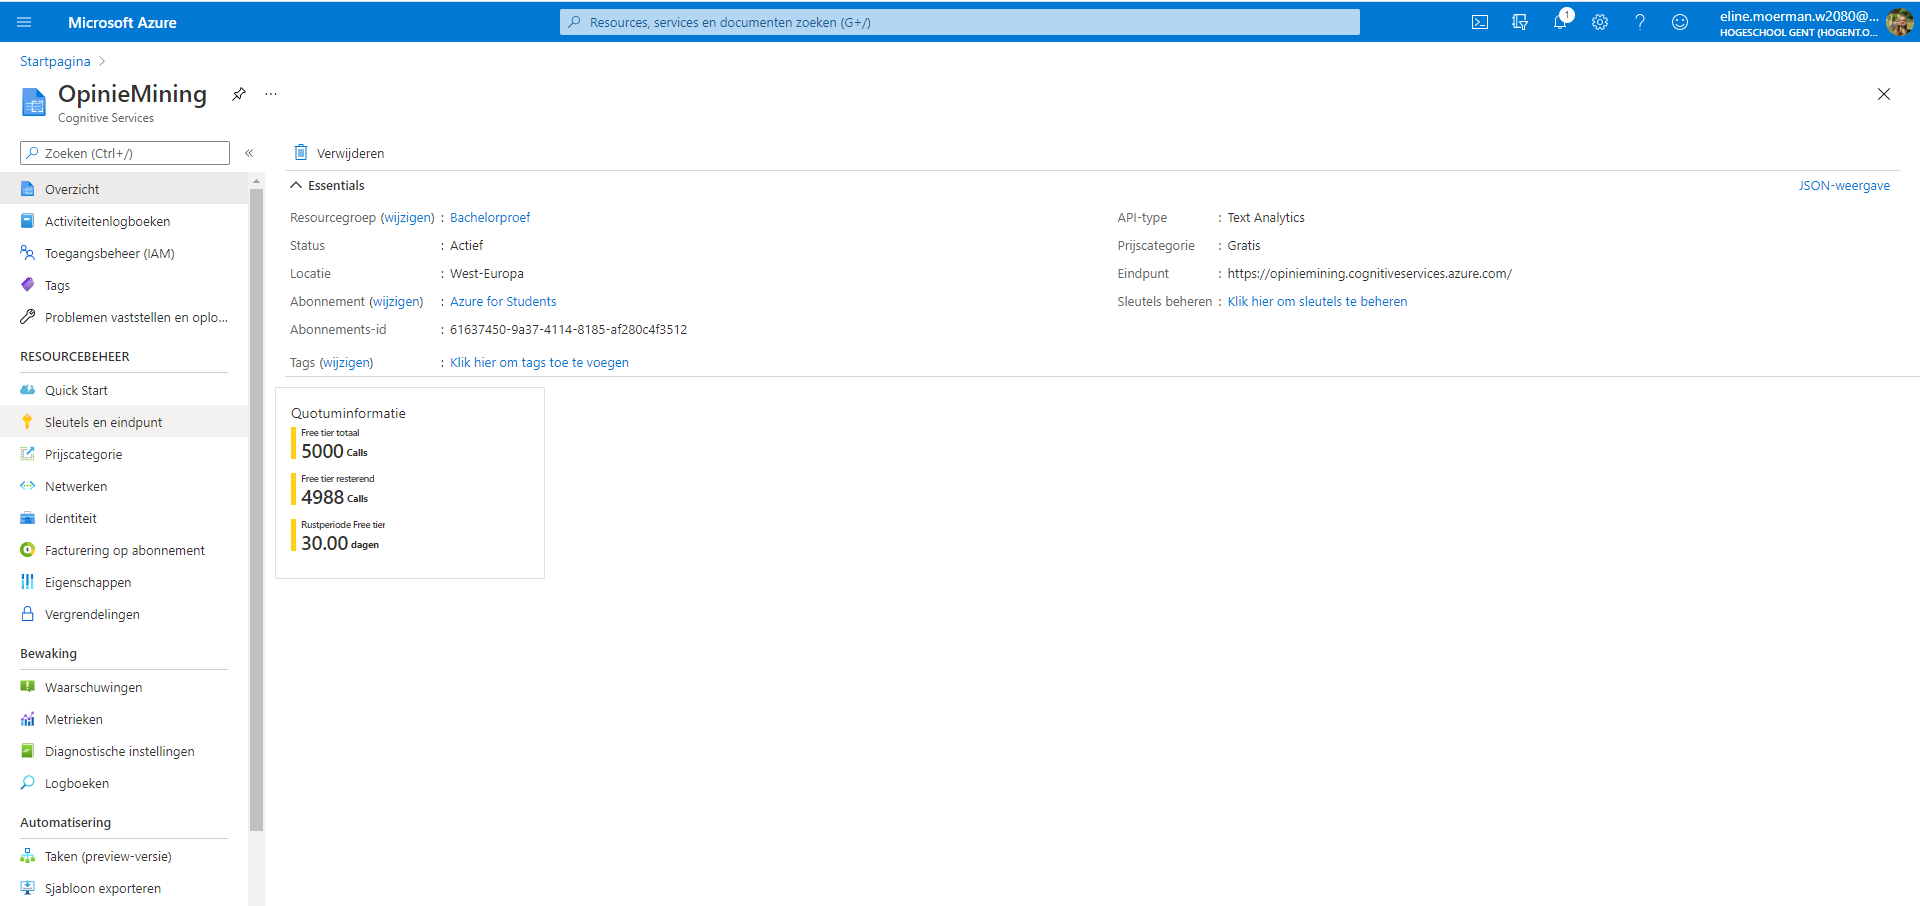
\includegraphics[width=\textwidth]{AzureResource.PNG}
    \caption{\label{azureresource}De Azure Text Analytics Resource \autocite{Microsoft2021}.}
\end{figure}
\FloatBarrier

Eenmaal dat de service aangemaakt is, genereert Azure een sleutel en een endpoint. Deze zullen gebruikt worden in Visual Studio om de Azure service te kunnen gebruiken. De key en endpoint zijn nodig zodat niemand anders van deze service kan gebruik maken. 

\textbf{Stap 2}: Een project opzetten in Visual Studio en de juiste packages installeren

Wanneer Visual Studio opgestart wordt, vraagt de applicatie om een nieuw project te maken. Hier is de beste keuze een .NET Core console applicatie. Dit zorgt ervoor dat er geen overbodige bestanden worden aangemaakt en dat we enkel de file Program.cs krijgen. In deze file zal al de code geschreven worden om de datasets te kunnen analyseren. \autocite{Microsoft2020}

Daarna moet er een package geïnstalleerd worden. Een package is herbruikbare code die al door andere developers geschreven zijn en die de gebruiker kan downloaden in zijn of haar project. \autocite{Microsoft2018} De package die nodig is is Azure.AI.TextAnalytics, zoals te zien op figuur 3.2.

\begin{figure}[!htbp]
    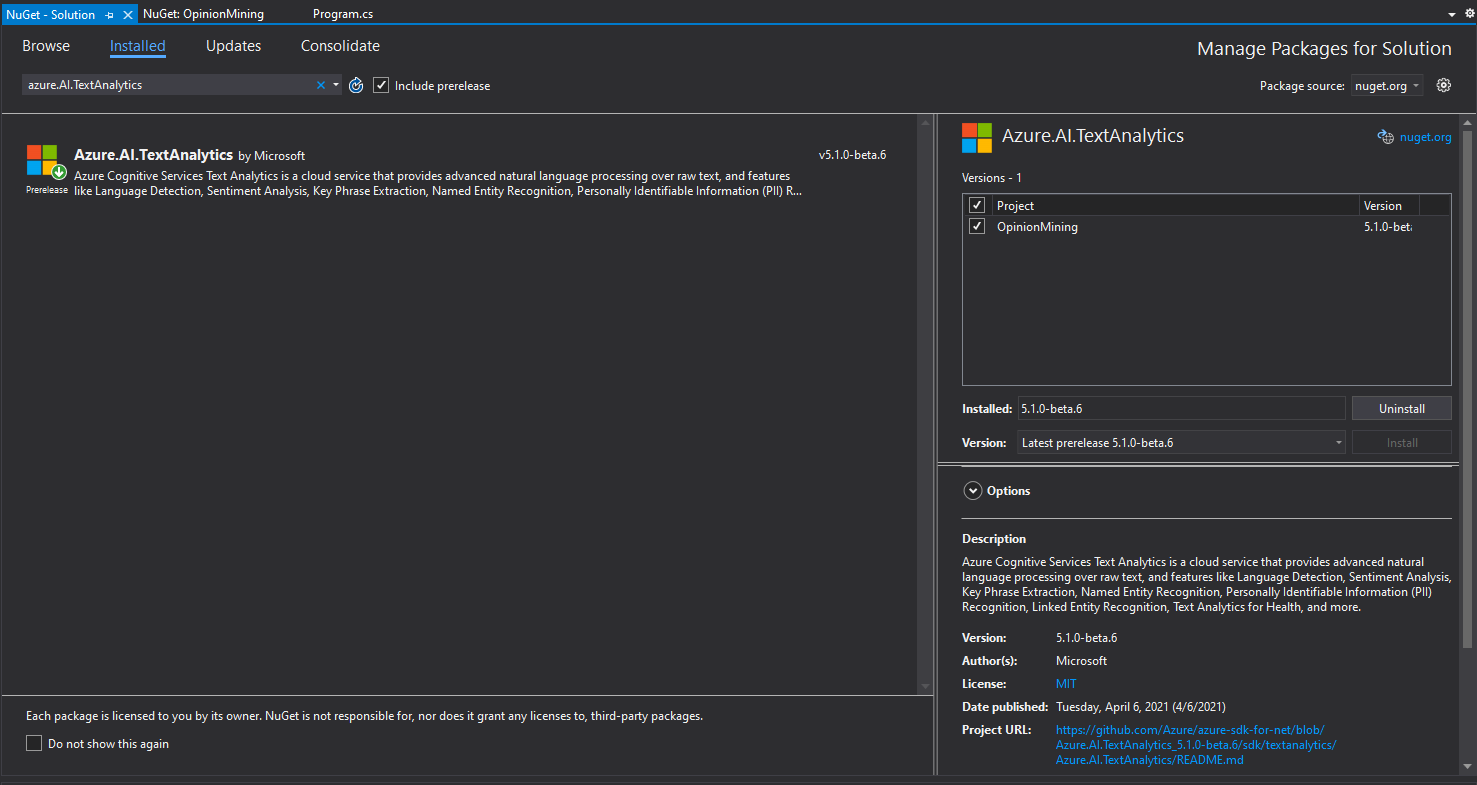
\includegraphics[width=\textwidth]{AzurePackage.PNG}
    \caption{\label{azurepackage}De Azure TextAnalytics Package \autocite{Microsoft2020}.}
\end{figure}
\FloatBarrier


\textbf{Stap 3}: De juiste code schrijven om zinnen te kunnen analyseren


\subsection{Amazon Dataset}
\label{amazondatasetazure}

\section{MonkeyLearn}

\subsection{Achtergrond informatie}
\label{achtergrondinformatiemonkeylearn}

\section{Proof Of Concept}

